% !Tex root = Article.tex
\documentclass[a4paper, 12pt]{article}

\usepackage[UTF-8]{ctex}
\usepackage{indentfirst}
\usepackage{amsmath}
\usepackage{tabularray}
\usepackage{xcolor}
\usepackage{listings}
\usepackage{subfigure}
\usepackage[graphicx]{realboxes}
\usepackage{diagbox}
\usepackage{multirow}

\lstset{
    basicstyle          =   \sffamily,
    keywordstyle        =   \bfseries,
    commentstyle        =   \rmfamily\itshape,
    stringstyle         =   \ttfamily,
    flexiblecolumns,
    numbers             =   left,
    showspaces          =   false,
    numberstyle         =   \zihao{-5}\ttfamily,
    showstringspaces    =   false,
    captionpos          =   t,
    frame               =   lrtb,
}

\lstdefinestyle{Python}{
    language        =   Python,
    basicstyle      =   \zihao{-5}\ttfamily,
    numberstyle     =   \zihao{-5}\ttfamily,
    keywordstyle    =   \color{blue},
    keywordstyle    =   [2] \color{teal},
    stringstyle     =   \color{magenta},
    commentstyle    =   \color{red}\ttfamily,
    breaklines      =   true,
    columns         =   fixed,
    basewidth       =   0.5em,
}

\setlength{\parindent}{2em}
\numberwithin{equation}{section}

\begin{document}

    \title{基于''层次分析法''和''灰色预测模型''的低碳建筑研究}
    \author{}
    \date{}
    \maketitle

    \centerline{\textbf{\LARGE{摘要}}}

    \textbf{\large{关键词}}

    {\centering{\section{问题重述}}}
        \subsection{问题背景}
        “双碳”即碳达峰与碳中和的简称,我国力争2030年前实现碳达峰,2060年前实现碳中和。
        “双碳”战略倡导绿色、环保、低碳的生活方式。我国加快降低碳排放步伐,大力推进绿色低碳科技创新,以提高产业和经济的全球竞争力。
        低碳建筑是指在建筑材料与设备制造、施工建造和建筑物使用的整个生命周期内,减少化石能源的使用,提高能效,降低二氧化碳排放量。

        \subsection{目标任务}
            \textbf{问题一:}计算给定建筑通过空调调节温度的年碳排放量。

            \textbf{问题二:}建立综合评价模型,找出易于量化的指标,评估居住建筑整个生命周期的碳排放。

            \textbf{问题三:}基于问题二,考虑建筑生命周期三个阶段的碳排放问题,对江苏省13个地级市的居住建筑进行评价,验证模型的有效性。

            \textbf{问题四:}建立碳排放预测模型,基于江苏省建筑全过程碳排放的历史数据,对2023年江苏省建筑全过程的碳排放量进行预测。

            \textbf{问题五:}结合前面的讨论给出江苏省建筑碳减排的政策建议。


    {\centering{\section{问题分析}}}
        \subsection{问题一}
            问题一要求计算空调调节温度产生的年碳排放量,又给出了碳排放量与用电量的关系,因此我们需要求出空调调节温度所用电量。
            为了进一步简化计算,我们假设室外温度始终为月平均温度,然后我们找出需要开空调的月份,并且规定开空调的目的是让温度维持在目标温度上届或下届。
            然后计算出空调制冷或制热所制造的热量,通过EER或COP算出空调消耗的电量,即达成目标,最后换算即可。

        \subsection{问题二}
            问题二要求选取指标构建评价模型评估居住建筑整个生命周期的碳排放。我们选择了使用层次分析法来构建评价模型,
            将指标作为准则层的准则,构建起层次分析法的框架。

        \subsection{问题三}
            问题三要求在问题二的基础上考虑建筑生命周期三个阶段的碳排放问题,对江苏省13个地级市的居住建筑进行评价并验证模型的可行性。
            因此我们在建筑的生命周期三个阶段各自选取了一些指标增加进问题二所构建模型的准则层中,将江苏省13个地级市的居住建筑生命周期碳排放量作为输入输入到模型中,
            将模型给出的评价分进行排序,与实际排名进行对比,进而判断模型的有效性。

        \subsection{问题四}
            问题四要求建立碳排放预测模型,基于江苏省建筑全过程碳排放的历史数据预测2023年江苏省建筑全过程碳排放。
            注意到数据和预测目标有数据量较少、预测目标较近期的特点,我们选择使用构建灰色预测GM (1, 1)模型作为预测模型。

        \subsection{问题五}
<<<<<<< HEAD
        经过以上分析,我们对江苏省建筑碳减排的政策的建议如下
=======
            经过以上分析,我们对江苏省建筑碳减排的政策的建议如下
>>>>>>> 9de725819d54d85e2847062dc208fdf995334f6e
            \begin{enumerate}
                \item 建筑设计标准:加强建筑能效等级和节能措施的规定,提高被动设计的实现率。鼓励使用绿色环保材料,减少建筑材料的使用量。
                \item 促进可再生能源利用:鼓励建筑采用太阳能、地源热泵等可再生能源设施,减少对传统能源的依赖,降低运行阶段的碳排放量。
                \item 改善建筑使用效率:推广智能化节能控制系统,优化空调、照明、通风等系统的运行方式,减少不必要的能源消耗。
                \item 推广低碳生活方式:鼓励居民采用低碳出行方式,如步行、骑行、乘坐公共交通工具等,减少个人碳排放量。
                \item 废弃物处理:鼓励采用回收利用的废弃物处理方式,减少拆除阶段的碳排放量。
                \item 建立碳排放权交易市场:通过建立碳排放权交易市场,引导企业和个人减少碳排放,实现碳排放量的交易和管理。
                \item 优化政策环境:加强碳排放标准的规定和执行力度,鼓励和支持低碳技术研发和应用。引导金融机构加大对低碳建筑项目的投资和支持力度。
                \item 把节约能源资源放在首位,实行全面节约战略,倡导推广绿色低碳的生产生活方式,大幅提高投入产出效率,持续降低单位产出能源资源消耗和碳排放,从源头和入口形成有效的碳排放控制阀门。
                \item 统筹省内外能源资源,推广先进绿色低碳技术和经验。推动省内应对气候变化对外合作有序开展,加强交流合作,不断提高参与度和影响力。
                \item 加强低碳社会建设宣传教育,提高全社会对碳达峰、碳中和的认知度和认可度。引导和支持各类市场主体适应低碳发展要求,提升低碳创新水平。以示范创建为载体,推广绿色低碳生产生活方式,扩大绿色低碳产品供给和消费,倡导形成简约适度、绿色低碳的生活方式。
                \item 政府和市场共同发挥作用,科技、产业和制度创新协同并进,增强原始创新支撑能力,加快全面数字化,深化能源等相关领域改革,形成有效激励约束机制,构建绿色低碳创新体系。
                \item 进工业低碳工艺革新、数字化转型和绿色制造体系建设,加快重点领域对照标杆水平实施节能降碳技术改造,鼓励国有企业、骨干企业开展示范性改造。
                \item 大力培育节能环保、资源循环利用、清洁能源等绿色低碳产业,聚焦集成电路、生物医药、人工智能等前沿领域,积极发展新一代信息技术、新材料、新能源汽车等战略性新兴产业。
            \end{enumerate}


    {\centering{\section{模型假设}}}
        \begin{enumerate}
            \item 假设建筑地面相当于厚度一米的导热层,假设门窗厚度为0.1m;
            \item 假设室外温度为月平均温度,假设空调只在室外温度不在目标温度区间时才开启;
            \item 假设开空调的目的是使温度保持在目标温度区间上界或下届(取接近一方),不考虑刚开关空调时室内温度逐渐上升或逐渐下降的情况;
            \item 假设各地区不同指标的碳排放为在该指标的得分,不考虑选定指标之外的碳排放;
        \end{enumerate}


    {\centering{\section{符号说明}}}
        \textbf{见上页表一。}
        \begin{table}[htbp]
            \centering
            \caption{符号说明}
            \begin{tabular}{c c c}
                \hline \hline \noalign{\smallskip}
                变量 & 定义 & 单位 \\
                \noalign{\smallskip} \hline \noalign{\smallskip}
                $ Q_{heat} $ & 空调制热产生热量 & \textit{J} \\
                $ Q_{cold} $ & 空调制冷产生热量 & \textit{J} \\
                $ Q_{make} $ & 空调总共产生热量 & \textit{J} \\
                $ Q_{elec} $ & 空调消耗电能 & \textit{J} \\
                $ t_{in} $ & 室内温度 & $ ^{\circ}C $ \\
                $ t_{out} $ & 室外温度 & $ ^{\circ}C $ \\
                $ t_{ave} $ & 月平均温度 & $ ^{\circ}C $ \\
                $ \Delta T $ & 室内外温差 & $ ^{\circ}C $ \\
                $ \Phi $ & 传热速率 & \textit{W} \\
                $ \lambda $ & 导热系数 & $ W / m^{2} \cdot K $ \\
                \textit{A} & 传热面积 & $ m^{2} $ \\
                $ \delta $ & 材料厚度 & \textit{m} \\
                \textit{W} & 权重向量 & / \\
                $ \lambda _{\max} $ & 最大特征值 & / \\
                \textit{T} & 最大特征值对应特征向量 & / \\
                \textit{CI} & 一致性指标 & / \\
                \textit{RI} & 平均随机一致性指标 & / \\
                \textit{CR} & 检验系数 & / \\
                \textit{P} & 评分矩阵 & / \\
                \textit{S} & 得分矩阵 & / \\
                $ x^{ (0)} $ & 年份-数据序列 & / \\
                $ x^{ (1)} $ & 累加生成序列 & / \\
                $ \lambda (k) $ & 关联系数 & / \\
                \textit{a} & 发展系数 & / \\
                \textit{u} & 灰色作用量 & / \\
                $ \hat{a} $ & 最佳近似发展系数 & / \\
                $ \hat{u} $ & 最佳近似灰色作用量 & / \\
                \textit{C} & 后验差比值 & / \\
                $ \sigma _{1} $ & 历史数据方差 & / \\
                $ \sigma _{2} $ & 残差方差 & / \\
                \noalign{\smallskip} \hline \noalign{\smallskip}
            \end{tabular}
        \end{table}


    {\centering{\section{模型的建立与求解}}}
        \subsection{问题一的模型建立与求解}
            问题一要求计算通过空题调节温度产生的年碳排放量。
            我们需先求出空调制热和制冷的热量,借此通过\textit{COP}和\textit{EER}求出空调消耗的电量,最后转换成碳排放。
            其中\textit{COP}和\textit{EER}的定义分别为
            \begin{equation}
                COP = \frac{Q_{heat}}{W},\hspace{2em} EER = \frac{Q_{cold}}{W}
            \end{equation}
            $ Q_{heat} / Q_{cold} $指的是单位时间内的制热/制冷量,单位为\textit{J},
            公式中\textit{W}指的是单位为时间内空调消耗的功率,单位为\textit{W}

            首先计算出建筑物各个月的能量需求量。设室内温度要维持的温度为 $ t_{in} $,室外温度为 $ t_{out} $,
            当月该地区平均温度为 $ t_{ave} $ ,方便起见,我们规定
            \begin{equation*}
                t_{out} = t_{ave}
            \end{equation*}
            \begin{equation*}
                t_{in} =
                \begin{cases}
                    18 ^{\circ}C & \text{ $ t_{out} < 18 ^{\circ}C $ } \\
                    t_{out} & \text{ $ t_{out} \in [18 ^{\circ}C, 26 ^{\circ}C] $ } \\
                    26 ^{\circ}C & \text{ $ t_{out} > 26 ^{\circ}C $}
                \end{cases}
            \end{equation*}

            我们使用热传导方程计算用来需要制热/制冷的热量,其形式为
            \begin{equation}
                \Phi = \frac{\lambda \cdot A \cdot |\Delta T|}{\delta}
            \end{equation}
            其中$ \Phi $表示传热速率,$ \lambda $为导热系数,\textit{A}为传热面积,
            $ \Delta T $是室内外温度差,即$ t_{in} - t_{out} $,$ \delta $表示材料厚度。

            将建筑分成墙、门窗、房顶、地面四个部分,分别计算并累加即可得到需要制热/制冷的热量,设为$ Q_{make} $,
            由\textit{COP}和\textit{EER}的定义可得到需电量$ Q_{elec} $和热量$ Q_{make} $的转化关系
            \begin{equation}
                Q_{elec} =
                \begin{cases}
                    \frac{Q_{make}}{EER} & \text{ $ \Delta t < 0 $ } \\
                    0 & \text{ $ \Delta t = 0 $ } \\
                    \frac{Q_{make}}{COP} & \text{ $ \Delta t > 0 $ }
                \end{cases}
            \end{equation}

            最后根据需电量与碳排放的换算关系 $ m = Q_{elec} \cdot 0.28 $ 求出每月碳排放后累加,即得到年度碳排放量。


        \subsection{问题二的模型建立与求解}
            \subsubsection{建立层次结构模型}
                \begin{figure}[h]
                    \centering
                    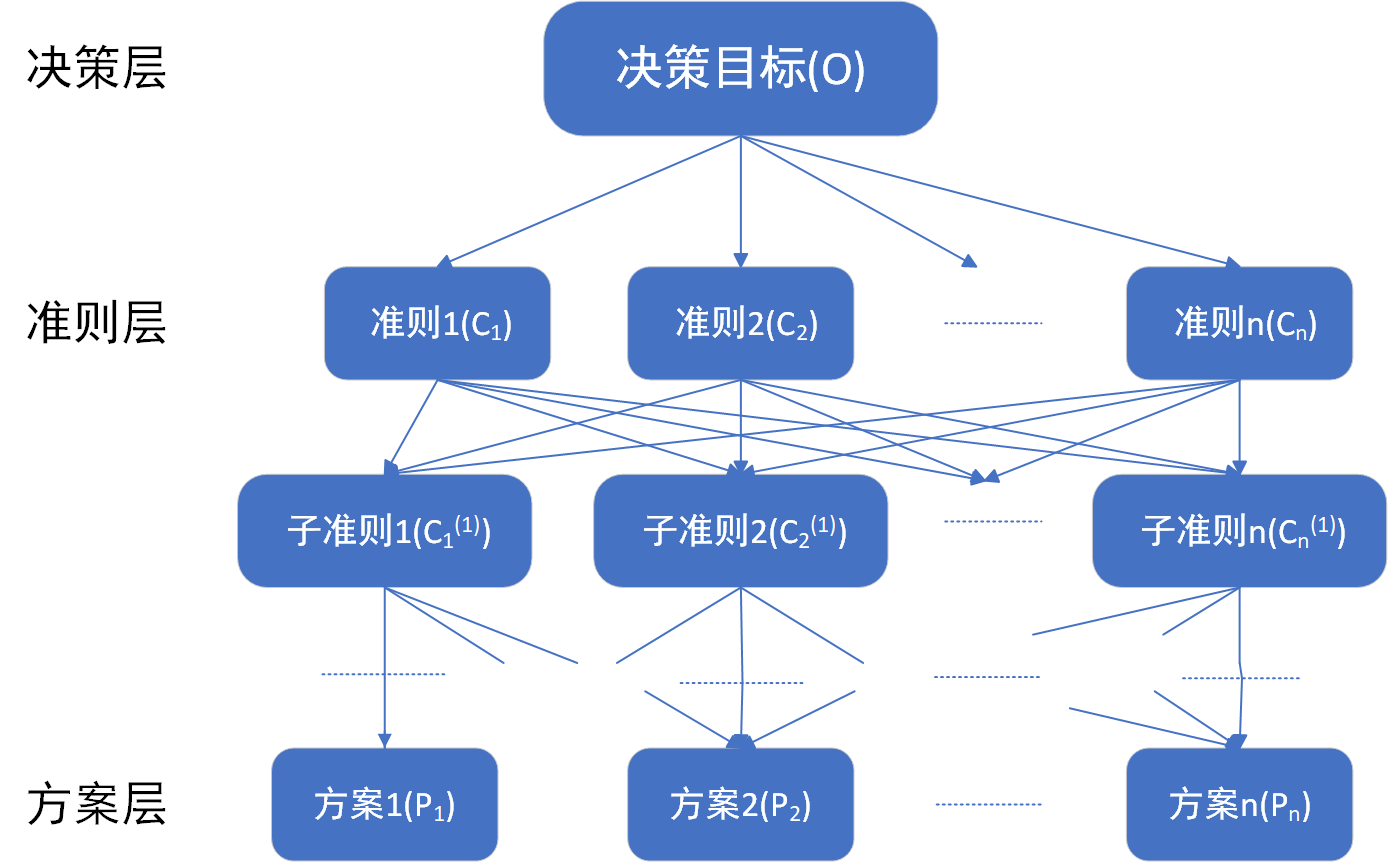
\includegraphics[height=4.5cm,width=9.5cm]{层次分析法框架.png}
                    \caption{层次分析法框架}
                \end{figure}
                准则层中准则因素之间相互独立。 \\
                我们选择的准则因素有:生活使用能耗、地区差异、周边产业、建造与拆除能耗、生产运输。


            \subsubsection{构建成对比较矩阵及归一化}
                \begin{enumerate}
                    \item 构建比较矩阵 \\
                        \qquad 构造比较矩阵是通过比较同一层次上的各因素对上–层相关因素的影响作用.而不是把所有因素放在一起比较,即将同一层的各因素进行两两对比。
                        设某层有n个因素,$ x = \{x_{1}, x_{2} \dots x_{n}\} $要比较它们对上一层某一准则 (或目标)的影响程度,确定在该层中相对于某一准则所占的比重。
                        上述比较是两两因素之间进行的比较,比较时常取1~9尺度。

                        \begin{table}[h]
                            \centering
                            \begin{tabular}{|c|c|} \hline
                                尺度 & 含义 \\ \hline
                                1 & 第i个因素与第j个因素影响相同 \\ \hline
                                3 & 第i个因素与第j个因素影响稍强 \\ \hline
                                5 & 第i个因素与第j个因素影响较强 \\ \hline
                                7 & 第i个因素与第j个因素影响明显强 \\ \hline
                                9 & 第i个因素与第j个因素影响极端强 \\ \hline
                                2, 4, 6, 8 & 两相邻判断的中间值 \\ \hline
                            \end{tabular}
                        \end{table}

                        用$ a_{ij} $表示第i个因素相对于第j个因素的比较结果,则
                        \[ a_{ij} = \frac{1}{a_{ji}} \]
                        \begin{equation}
                            A = (a_{ij})_{n \times n} =
                            \begin{pmatrix}
                                a_{11} & a_{12} & \cdots & a_{1n} \\
                                a_{21} & a_{22} & \cdots & a_{2n} \\
                                \cdots & \cdots & \cdots & \cdots \\
                                a_{n1} & a_{n2} & \cdots & a_{nn}
                            \end{pmatrix}
                        \end{equation}

                        A则称为成对比较矩阵。

                        \newpage

                        \item 归一化 \\
                            对各城市的数据进行归一化处理
                            \begin{table}[h]
                                \centering
                                \begin{tabular}[h]{|l|c|c|c|c|c|} \hline
                                    \diagbox{指标}{数据}{城市} & 苏州 & 南京 & 南通 & 无锡 & 常州 \\ \hline
                                    直接 & 48 & 51.5 & 27 & 57.2 & 29 \\ \hline
                                    间接 & 126.3 & 134.3 & 118.7 & 97.8 & 71.6 \\ \hline
                                    运营 & 4.8 & 4.9 & 3.5 & 2.7 & 2.8 \\ \hline
                                    \multirow{3}{*}{归一化比例} & 0.226 & 0.242 & 0.127 & 0.269 & 0.126 \\ \cline{2-6}
                                    ~ & 0.230 & 0.245 & 0.216 & 0.178 & 0.130 \\ \cline{2-6}
                                    ~ & 0.257 & 0.262 & 0.187 & 0.144 & 0.150 \\ \hline
                                \end{tabular}
                            \end{table}
                    \end{enumerate}


                \subsubsection{层次单排序及一致性检验}
                    \begin{enumerate}
                        \item 层次单排序 \\
                            \textbf{和积法}(算术平均法):取判断矩阵\textit{n}个列向量归一化后的算术平均值,近似作为权重,即
                            \begin{equation}
                                W_{i} = \frac{1}{n} \sum_{j=1}^{n} \frac{a_{ij}}{\sum_{k=1}^{n} a_{kj}} (i = 1, 2, \cdots, n)
                            \end{equation}

                            \textbf{求根法}(几何平均法):将比较矩阵的各列(或行)向量求几何平均后归一化,可近似作权重,即
                            \begin{equation}
                                W_{i} = \sum_{j=1}^{n} \frac{(\prod_{j=1}^{n} a_{ij})_{\frac{1}{n}}}{\sum_{k=1}^{n} (\prod_{j=1}^{n})_{\frac{1}{n}}} (i = 1, 2, \cdots, n)
                            \end{equation}

                            \textbf{特征值法}:求出矩阵的最大特征值$ \lambda _{\max} $以及其对应的特征向量\textit{T},对求出的特征向量进行归一化即可得到我们的权重。

                            在我们的模型中综合采用了三种方法得到权重,降低了单一方法带来的不确定性,使数据结果更加可靠。


                        \item 一致性检验 \\
                        通常情况下,由实际得到的判断矩阵不一定是一致的,即不一定满足传递性和一致性实际中,也不必要求一致性绝对成立,
                        但要求大体上是一致的,即不一致的程度应在容许的范围内主要考查以下指标:
                            \begin{enumerate}
                                \item 一致性指标\textit{CI}
                                    \begin{equation}
                                        CI = \frac{\lambda _{\max} - n}{n - 1}
                                    \end{equation}

                                \item 平均随机一致性指标\textit{RI} \\
                                    为衡量\textit{CI}的大小,引入随机一致性指标\textit{RI}:
                                    \begin{equation}
                                        RI = \frac{CI_{1} + CI_{2} + \cdots + CI_{n}}{n}
                                    \end{equation}
                                    其中,随机一致性指标\textit{RI}和判断矩阵的阶数有关,一般情况下,
                                    矩阵阶数越大,则出现一致性随机偏离的可能性也越大,对于阶数小于9,其对应关系如图:
                                    \begin{table}[h]
                                        \centering
                                        \begin{tabular}{l|c c c c c c c c c} \hline
                                            \textit{n} & 1 & 2 & 3 & 4 & 5 & 6 & 7 & 8 & 9 \\ \hline
                                            \textit{RI} & 0 & 0 & 0.58 & 0.90 & 1.12 & 1.24 & 1.32 & 1.41 & 1.45 \\ \hline
                                        \end{tabular}
                                    \end{table}

                                \item 检验系数\textit{CR} \\
                                    考虑到一致性的偏离有可能是由于随机原因造成的,因此在检验判断矩阵是否具有满意的一致性时,
                                    还需将\textit{CI}和\textit{RI}进行比较,得出检验系数\textit{CR},公式如下:
                                    \begin{equation}
                                        CR = \frac{CI}{RI}
                                    \end{equation}
                                    一般地,如果$ CR \le 0.1 $,则认为该判断矩阵通过一致性检验,$ A_{\max} $对应的特征向量\textit{W}可以作为排序的权重向量,此时
                                    \begin{equation}
                                        \lambda _{\max} \approx \sum_{i=1}^{n} \frac{ (A \cdot W)_{i}}{nw_{i}} = \frac{1}{n} \sum_{i=1}^{n} \frac{\sum_{j=1}^{n} a_{ij}w_{j}}{w_{i}}
                                    \end{equation}
                                    否则就不具有满意一致性,需要调整对比较矩阵。
                            \end{enumerate}
                    \end{enumerate}


                \subsubsection{计算组合权重及得分}
                    得到最大特征值对应的特征向量
                    \[ T = [t_1 \quad t_2 \quad \cdots \quad t_n] \]
                    \newline
                    计算得到权重向量
                    \[ W = [w_1 \quad w_2 \quad \cdots \quad w_n ] \]
                    \begin{equation*}
                        w_i = \frac{t_i}{\sum_{i=1}^{n} t_i}
                    \end{equation*}
                    \newline
                    随后分别通过公式 (5.2)和公式 (5.3)求得两个权重向量, 最后将三个权重向量取算术平均作为最终的权重向量。
                    设指标评分矩阵为\textit{P},那么最后的得分矩阵\textit{S}为:
                    \[ S = P \cdot W \]


            \subsection{问题三的模型建立与求解}
                \subsubsection{模型的建立}
                    基于第二问所建模型,通过建筑生命周期的三个阶段确定代表性强的指标加入模型评价。我们选取的指标有: \\
                    \textit{建造阶段:建筑材料生产运输的碳排放系数、建造过程所产生的碳排放} \\
                    \textit{运行阶段:生活使用能耗、气候原因、地区差异、周边产业} \\
                    \textit{建造阶段:拆除过程的能耗}

                \subsubsection{模型的验证}
                    为了验证模型的有效性,我们将2021年江苏省13个地级市的居住建筑碳排放作为输入输入到所建立模型中进行综合评价,
                    并将得到的结果排名与实际的排名进行比较,结果如图:
                    \newpage
                    \begin{figure}[h]
                        \centering
                        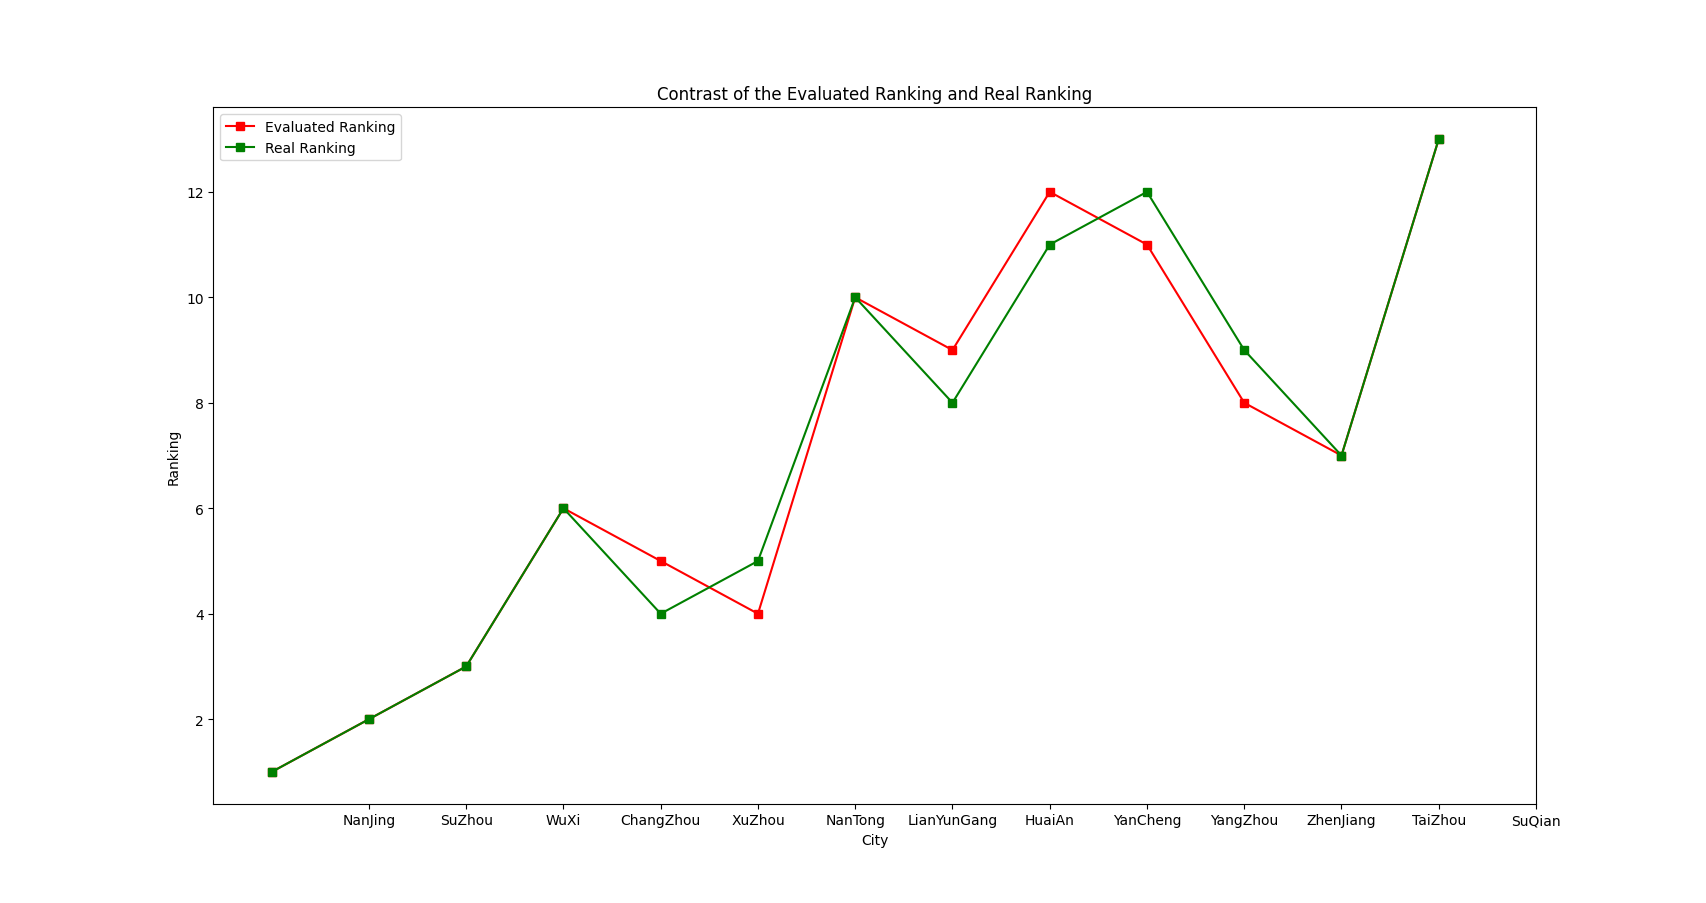
\includegraphics[height=9cm,width=15cm]{contrast_q3.png}
                        \caption{CONTRAST}
                    \end{figure}
                    通过比较来看,评价模型的评价结果与实际结果吻合得较好,很好的验证了所建立模型的有效性。


            \subsection{问题四的模型建立与求解}
                \subsubsection{模型的分析}
                    本题是分析预测2023年江苏省建筑全过程的碳排放量。
                    由于要求基于江苏省建筑全过程碳排放的历史数据建立预测模型,用于分析江苏省未来建筑全过程的碳排放量,
                    因此我们采用信息不完全、不充分的预测系统——灰色预测,建立灰色预测模型GM (1,1)模型,基于历史时期数据去预测未来时期数据。

                \subsubsection{模型的建立}
                    \begin{enumerate}
                        \item \textbf{级比检验} \\
                            级比检验用于判断数据序列进行模型构建的适用性,如果通过了该检验,则可以使用灰色预测。
                            计算公式为:
                            \begin{equation}
                                \lambda (k) = \frac{x^{ (0)} (k - 1)}{x^{ (0)} (k)}, k = 2, 3, \ldots, n
                            \end{equation}
                            如果$ \lambda (k) $在区间
                            \[ (e^{-\frac{2}{n + 1}}, e^{\frac{2}{n + 2}}) \]
                            内,说明可用GM (1,1)模型,其中$ x^{ (0)} (t) $ 是 \textit{年份-数据}序列。

                            如果$ \lambda (k) $在该区间外,则可尝试通过平移变换,将每个数据都加上某一常数\textit{c},
                            再看$ \lambda (k) $是否在区间内,最后模型结果再减去\textit{c}即可.
                            如果无论如何进行平移变换$ \lambda (k) $始终在该区间外,则说明该问题不适合用GM (1, 1)。

                            而经过计算,我们的数据可以通过级比检验。

                        \item \textbf{构造累加生成序列} \\
                            由于历史数据量少且无明显规律,难以预测,我们使用累加生成法得到一个新的序列$ x^{ (1)} (t) $,
                            并尝试用数学方法拟合新序列进而预测。累加生成序列公式为:
                            \begin{equation}
                                x^{ (1)} (k) = \sum_{i=1}^{k} x^{ (0)} (i)
                            \end{equation}

                        \item \textbf{构建一阶常微分方程} \\
                            通常情况下,累加生成序列的图像可用指数函数图像拟合,而一阶常微分方程的通解形式恰是指数函数,
                            因此我们构建一阶常微分方程,通过求解这个方程得到预测函数。 \\
                            该一阶常微分方程的形式为:
                            \begin{equation}
                                \frac{dx^{ (1)}}{dt} + ax^{ (1)} = u
                            \end{equation}
                            其中\textit{a, u}为\textit{发展系数}和\textit{灰色作用量}。
                    \end{enumerate}


                \subsubsection{模型的求解}
                    \begin{enumerate}
                        \item \textbf{方程式改写} \\
                            由于数据是离散而非连续的,首先将$ \frac{dx^{ (1)}}{dt} $改写成$ \frac{\Delta x^{ (1)}}{\Delta t} $。
                            而由于\textit{t}的单位是年份,因此始终有$ \Delta t = (t + 1) - t = 1 $,因此我们得到新形式的方程 \\
                            \[ x^{ (0)} (t) + ax^{ (1)} (t) = u \]
                            移项得到:
                            \begin{equation}
                                x^{ (0)} (t) = -ax^{ (1)} (t) + u
                            \end{equation}
                            得到该方程后,注意到可以通过最小二乘法求得最佳的参数\textit{a}和\textit{u}。


                        \item \textbf{最小二乘法求解最佳参数} \\
                            方程 (5.14)的矩阵形式为$ Y = BU $,具体形式为:
                            \begin{equation}
                                \begin{bmatrix}
                                    x^{ (0)} (2) \\
                                    x^{ (0)} (3) \\
                                    \vdots \\
                                    x^{ (0)} (N)
                                \end{bmatrix}
                                =
                                \begin{bmatrix}
                                    -\frac{1}{2} [ x^{ (1)} (2) + x^{ (1)} (1) & 1] \\
                                    -\frac{1}{2} [ x^{ (1)} (3) + x^{ (1)} (2) & 1] \\
                                    \vdots & 1 \\
                                    -\frac{1}{2} [ x^{ (1)} (N) + x^{ (1)} (N - 1) & 1]
                                \end{bmatrix}
                                \begin{bmatrix}
                                    a \\
                                    u
                                \end{bmatrix}
                            \end{equation}

                            我们要最小二乘法要求解的目标就是$ (Y - BU)^{T}(Y - BU) $取最小时的\textit{U}。
                            求解\textit{U}的估计值的方法为
                            \[ \hat{U} = [\hat{a}, \hat{u}] = (B^{T}B)^{-1}B^{T}Y \]
                            借此求得参数\textit{a, u}的最佳近似值$ \hat{a}, \hat{u} $后,即可求解微分方程得到拟合函数。


                        \item \textbf{求解微分方程} \\
                            通过方才求解到的$ \hat{a}, \hat{u} $,代入方程 (5.14),求得方程的解:
                            \begin{equation}
                                \hat{x}^{(1)} (k + 1) = (x^{(0)}(1) - \frac{\hat{u}}{\hat{a}})e^{-\hat{a}k} + \frac{\hat{u}}{\hat{a}}, \quad k = 0, 1, \cdots
                            \end{equation}
                            当\textit{k}小于已有数据量是,求得的为拟合值,大于时则是预测值。
                            需要注意的是求得的为$ \hat{x}^{(1)} $是累加生成序列,真正要求的原始序列$ \hat{x}^{(0)} $需要再通过差分法求得,即:
                            \begin{equation}
                                \hat{x}^{(0)}(k) =
                                \begin{cases}
                                    \hat{x}^{(1)}(1) & k = 1 \\
                                    \hat{x}^{(1)}(k) - \hat{x}^{(1)}(k - 1) & k > 1
                                \end{cases}
                            \end{equation}
                    \end{enumerate}


                \subsubsection{模型的检验}
                    最后需要对我们的模型进行检验,判断拟合值是否能较好地逼近实际值。常用的检验方法有:\textit{级比偏差检验、残差检验、后验差比检验等}。\\
                    我们选择的方法是后验差比检验,通过后验差比值\textit{C}的大小来判断模型的预测精度,其计算公式为:
                    \begin{equation}
                        C = \frac{\sigma _{1}}{\sigma _{2}}
                    \end{equation}
                    其中$ \sigma _{1}, \sigma _{2} $分别表示历史数据方差和残差方差。 \\
                    若\textit{C}值小于0.35,则可说明模型精度高;若小于0.5,则说明模型精度合格;若小于0.65,则说明模型精度基本合格;若大于0.65,则说明模型精度不合格。


                \subsubsection{模型结果}
                    模型拟合结果与预测和历史记录对比图如下:
                    \begin{figure}[h]
                        \centering
                        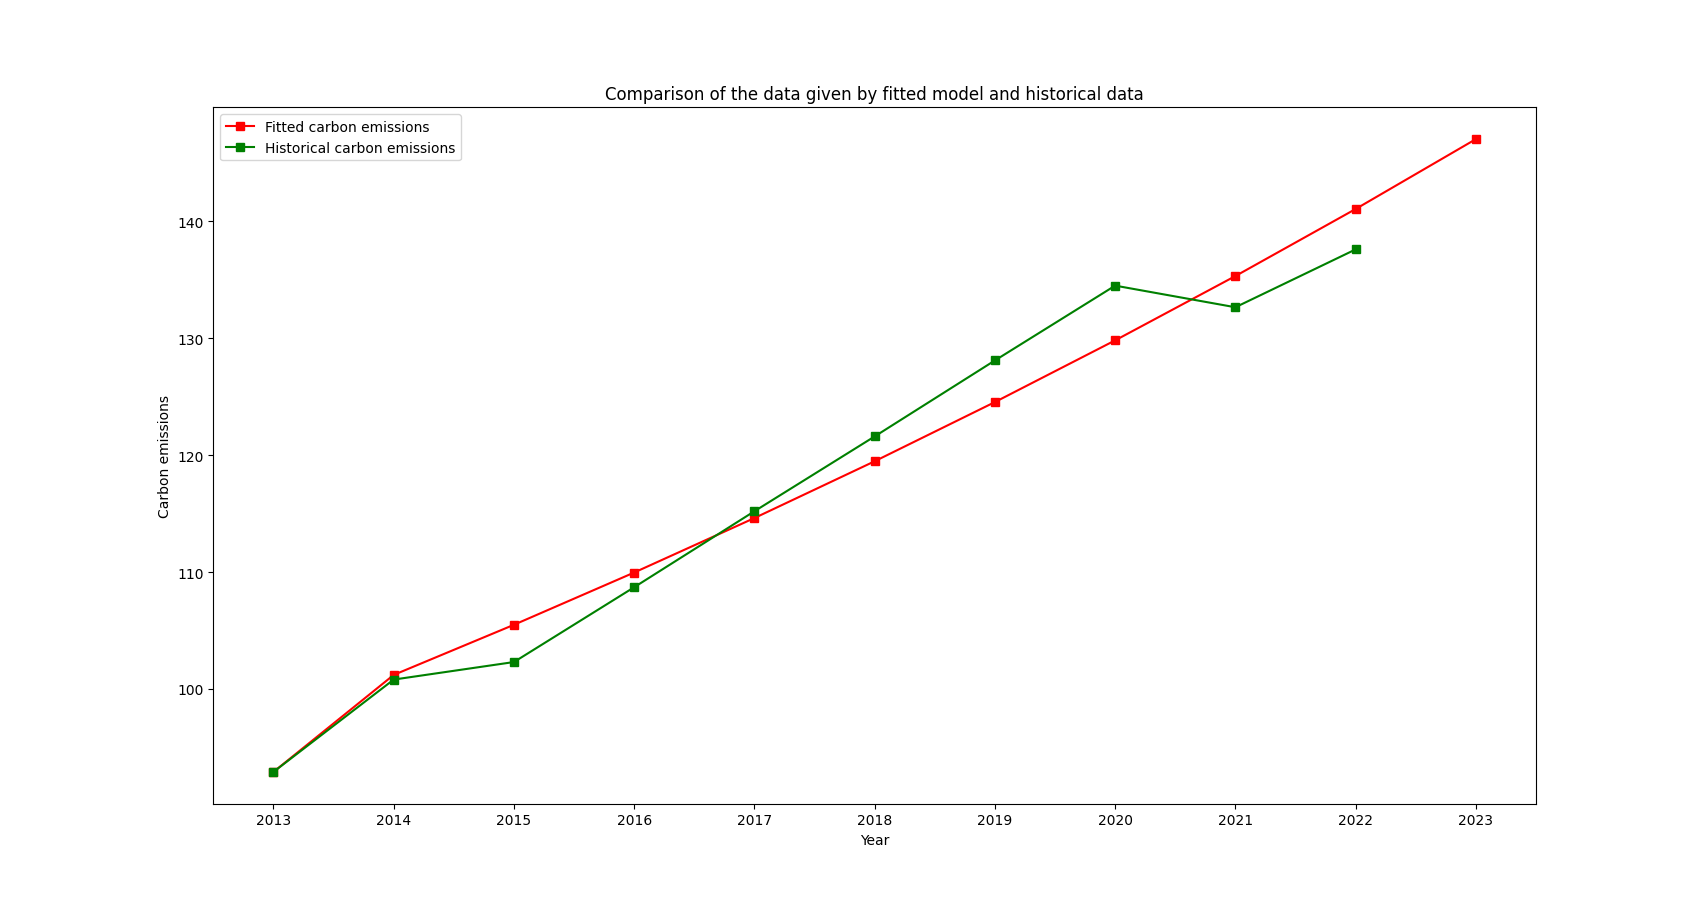
\includegraphics[height=9cm,width=15cm]{fit_and_his_q4.png}
                        \caption{COMPARISON}
                    \end{figure}

    {\centering{\section{结果检验与误差分析}}}


    {\centering{\section{模型评价}}}


    {\centering{\section{模型推广与改进}}}
        \subsection{预测模型的改进}
            \subsubsection{方程式修正}
                考虑到原方程中含有$ \frac{\Delta x^{ (1)}}{\Delta t} $,
                因此将$ x^{ (1)} (t) $修正为均值生成序列$ z^{ (1)} (t) $,计算公式为
                \[ z^{ (1)} (t) = \frac{x^{ (1)} (t)}{2} + \frac{x^{ (1)} (t - 1)}{2} + \cdots, \quad t = 2, \ldots, n \]
                即方程改写为
                \[ x^{ (0)} (t) = -az^{ (1)} (t) + u \]

            \subsubsection{检验改进}
                为进一步检验模型精度,最后的模型检验可使用多重方法检验模型精度。


    {\centering{\section{参考文献}}}
    \newpage


    {\centering{\section{附录}}}
        \subsection*{附录A \hspace{2em} 问题一}
            \lstinputlisting[
                style       =   Python,
                caption     =   {\bf Question1},
                label       =   {Question1.py}
            ]{Question1.py}

        \subsection*{附录B \hspace{2em} 问题二}
            \lstinputlisting[
                style       =   Python,
                caption     =   {\bf Question2},
                label       =   {Question2.py}
            ]{Question2.py}

        \subsection*{附录C \hspace{2em} 问题三}
            \lstinputlisting[
                style       =   Python,
                caption     =   {\bf Question3},
                label       =   {Question3.py}
            ]{Question3.py}

        \subsection*{附录D \hspace{2em} 问题四}
            \lstinputlisting[
                style       =   Python,
                caption     =   {\bf Question4},
                label       =   {Question4.py}
            ]{Question4.py}

\end{document}
